%
% @author   Shmish  "shmish90@gmail.com"
% @legal    MIT     "(c) Christopher Schmitt"
%


\documentclass{article}


%
% Document Imports
%

\usepackage{fancyhdr}
\usepackage{extramarks}
\usepackage{amsmath}
\usepackage{amssymb}
\usepackage{amsthm}
\usepackage{amsfonts}
\usepackage{algpseudocode}
\usepackage[table,xcdraw]{xcolor}
\usepackage{color}
\usepackage{tikz}
\usepackage{forest}
\usepackage{listings}
\usepackage{karnaugh-map}
\usepackage{graphicx}


\definecolor{dkgreen}{rgb}{0,0.6,0}
\definecolor{gray}{rgb}{0.5,0.5,0.5}
\definecolor{mauve}{rgb}{0.58,0,0.82}


\lstset{
  frame=tb,
  language=Verilog,
  aboveskip=3mm,
  belowskip=3mm,
  showstringspaces=false,
  columns=flexible,
  basicstyle=\ttfamily,
  numbers=none,
  numberstyle=\tiny\color{gray},
  keywordstyle=\color{blue},
  commentstyle=\color{dkgreen},
  stringstyle=\color{mauve},
  breaklines=true,
  breakatwhitespace=true,
  tabsize=3
}


%
% Document Configuation
%

\newcommand{\hwAuthor}{Christopher Schmitt}
\newcommand{\hwSubject}{CS 354}
\newcommand{\hwSection}{Section 02}
\newcommand{\hwSemester}{Fall 2019}
\newcommand{\hwAssignment}{Assignment 1}


%
% Document Enviornments
%

\setlength{\headheight}{65pt}
\pagestyle{fancy}
\lhead{\hwAuthor}
\rhead{
  \hwSubject \\
  \hwSection \\
  \hwSemester \\
  \hwAssignment
}

\newenvironment{problem}[1]{
  \nobreak\section*{Problem #1}
}{}


%
% Document Start
%

\begin{document}
  \begin{problem}{1}
    The majority function produces a false value when $\frac{n}{2}$ of the
    provided inputs are false (where $n$ is the number of inputs).  This
    function can be trivially implemented using three AND gates and two OR
    gates.

    \begin{center}
      \begin{math}
        \begin{array}{ccc|c}
          a&b&c&sum\\\hline
          0&0&0&\mathbf{0}\\
          0&0&1&\mathbf{0}\\
          0&1&0&\mathbf{0}\\
          0&1&1&\mathbf{1}\\
          1&0&0&\mathbf{0}\\
          1&0&1&\mathbf{1}\\
          1&1&0&\mathbf{1}\\
          1&1&1&\mathbf{1}
        \end{array}
      \end{math}
    \end{center}

    \begin{center}
      \begin{karnaugh-map}[4][2][1][$bc$][$a$]
        \minterms{3, 5, 6, 7}
        \maxterms{0, 1, 2, 4}
        \implicant{3}{7}
        \implicant{5}{7}
        \implicant{7}{6}
      \end{karnaugh-map}
    \end{center}

    \begin{center}
      \lstinputlisting{src/majority.v}
    \end{center}

    \begin{center}
      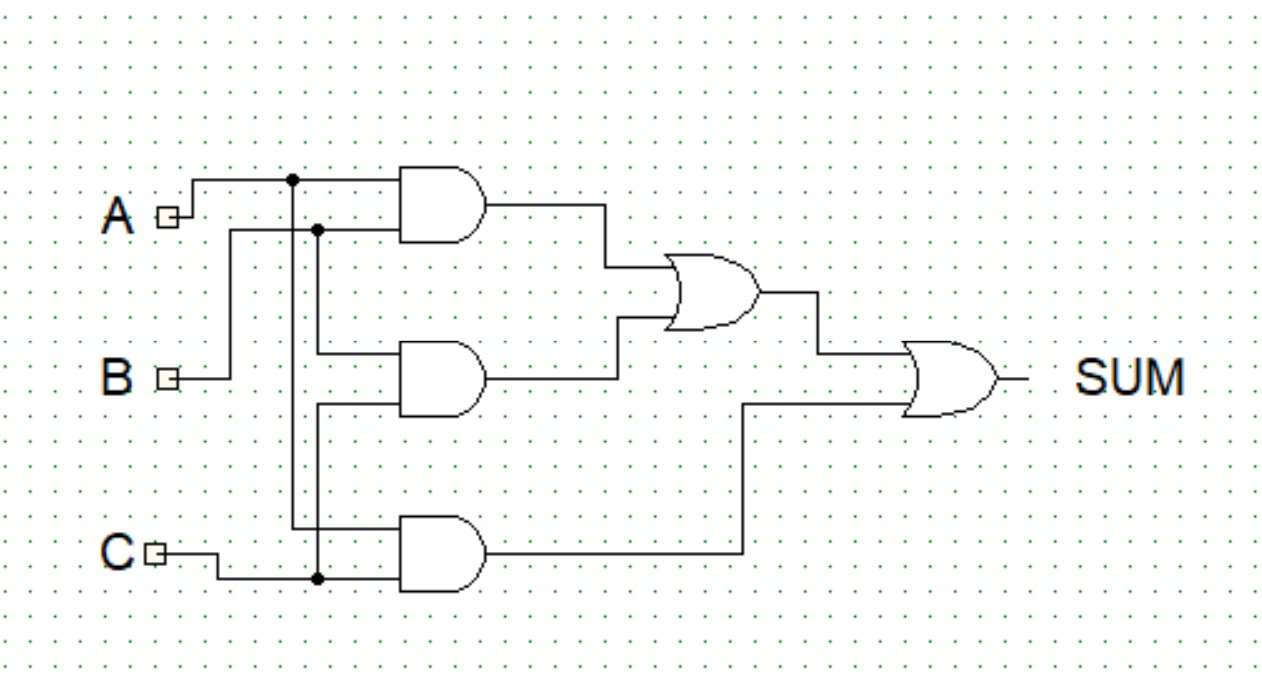
\includegraphics[scale=0.8]{images/majority.jpg}
    \end{center}

    \begin{center}
      \begin{lstlisting}
        iverilog.exe src/majority.v && vvp.exe a.out
        a = 0, b = 0, c = 0, sum = 0
        a = 0, b = 0, c = 1, sum = 0
        a = 0, b = 1, c = 0, sum = 0
        a = 0, b = 1, c = 1, sum = 1
        a = 1, b = 0, c = 0, sum = 0
        a = 1, b = 0, c = 1, sum = 1
        a = 1, b = 1, c = 0, sum = 1
        a = 1, b = 1, c = 1, sum = 1
      \end{lstlisting}
    \end{center}
  \end{problem}


  \begin{problem}{2}
    A conditional inverter is an XOR gate with exactly two unique inputs.  It,
    like all functions, can be broken down into ANDs, ORs, and NOTs.

    \begin{center}
      \begin{math}
        \begin{array}{cc|c}
          a&b&out\\\hline
          0&0&\mathbf{0}\\
          0&1&\mathbf{1}\\
          1&0&\mathbf{1}\\
          1&1&\mathbf{0}
        \end{array}
      \end{math}
    \end{center}

    \begin{center}
      \begin{karnaugh-map}[2][2][1][$b$][$a$]
        \minterms{1, 2}
        \maxterms{0, 3}
        \implicant{1}{1}
        \implicant{2}{2}
      \end{karnaugh-map}
    \end{center}

    \begin{center}
      \lstinputlisting{src/inverter.v}
    \end{center}

    \begin{center}
      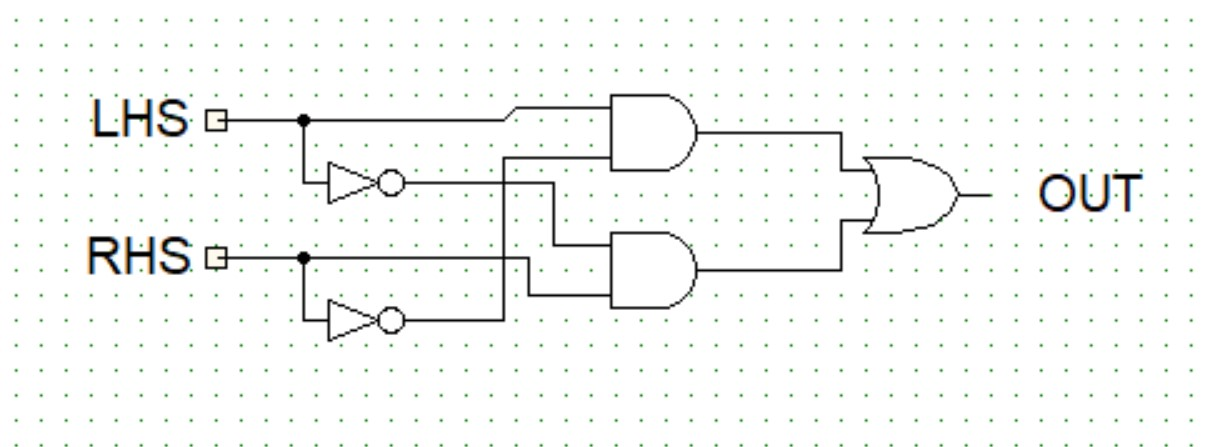
\includegraphics[scale=0.8]{images/inverter.jpg}
    \end{center}

    \begin{center}
      \begin{lstlisting}
        iverilog.exe src/inverter.v && vvp.exe a.out
        lhs = 0, rhs = 0, out = 0
        lhs = 0, rhs = 1, out = 1
        lhs = 1, rhs = 0, out = 1
        lhs = 1, rhs = 1, out = 0
      \end{lstlisting}
    \end{center}
  \end{problem}


  \begin{problem}{3}
    A simple two input multiplexer is a $2 \times 1$ multiplexer where $a$ and
    $b$ are inputs and $c$ is the control.  This function can be implemented
    easily using only AND, OR, and NOT gates.
    
    \begin{center}
      \begin{math}
        \begin{array}{ccc|c}
          a&b&c&out)\\\hline
          0&0&0&\mathbf{0}\\
          0&0&1&\mathbf{0}\\
          0&1&0&\mathbf{0}\\
          0&1&1&\mathbf{1}\\
          1&0&0&\mathbf{1}\\
          1&0&1&\mathbf{0}\\
          1&1&0&\mathbf{1}\\
          1&1&1&\mathbf{1}
        \end{array}
      \end{math}
    \end{center}

    \begin{center}
      \begin{karnaugh-map}[4][2][1][$bc$][$a$]
        \minterms{3, 4, 6, 7}
        \maxterms{0, 1, 2, 5}
        \implicant{3}{7}
        \implicantedge{4}{4}{6}{6}
      \end{karnaugh-map}
    \end{center}

    \begin{center}
      \lstinputlisting{src/multiplexer.v}
    \end{center}

    \begin{center}
      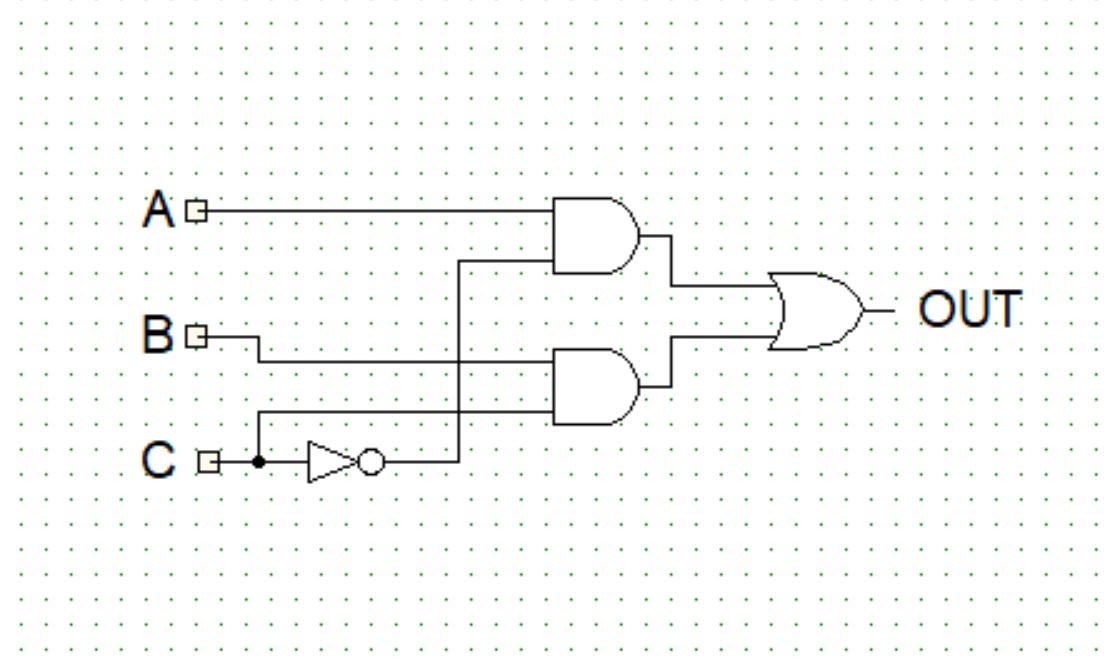
\includegraphics[scale=0.8]{images/multiplexer.jpg}
    \end{center}

    \begin{center}
      \begin{lstlisting}
        iverilog.exe src/multiplexer.v && vvp.exe a.out
        a = 0, b = 0, c = 0, out = 0
        a = 0, b = 0, c = 1, out = 0
        a = 0, b = 1, c = 0, out = 0
        a = 0, b = 1, c = 1, out = 1
        a = 1, b = 0, c = 0, out = 1
        a = 1, b = 0, c = 1, out = 0
        a = 1, b = 1, c = 0, out = 1
        a = 1, b = 1, c = 1, out = 1
      \end{lstlisting}
    \end{center}
  \end{problem}


  \begin{problem}{4}
    The one bit half adder is a circuit with two inputs and two outputs.  It
    computes both the sum and the carry given both the left and right hand
    sides as binary inputs.  The construction of this circuit can be greatly
    simplified through the use of an XOR gate.

    \begin{center}
      Sum (conditional inverter)
    \end{center}

    \begin{center}
      \begin{math}
        \begin{array}{cc|c}
          a&b&sum\\\hline
          0&0&\mathbf{0}\\
          0&1&\mathbf{1}\\
          1&0&\mathbf{1}\\
          1&1&\mathbf{0}
        \end{array}
      \end{math}
    \end{center}

    \begin{center}
      \begin{karnaugh-map}[2][2][1][$b$][$a$]
        \minterms{1, 2}
        \maxterms{0, 3}
        \implicant{1}{1}
        \implicant{2}{2}
      \end{karnaugh-map}
    \end{center}

    \begin{center}
      Carry (AND)
    \end{center}

    \begin{center}
      \begin{math}
        \begin{array}{cc|c}
          a&b&Carry\\\hline
          0&0&\mathbf{0}\\
          0&1&\mathbf{0}\\
          1&0&\mathbf{0}\\
          1&1&\mathbf{1}
        \end{array}
      \end{math}
    \end{center}

    \begin{center}
      \begin{karnaugh-map}[2][2][1][$b$][$a$]
        \minterms{3}
        \maxterms{0, 1, 2}
        \implicant{3}{3}
      \end{karnaugh-map}
    \end{center}

    \begin{center}
      \lstinputlisting{src/one_bit_half_adder.v}
    \end{center}

    \begin{center}
      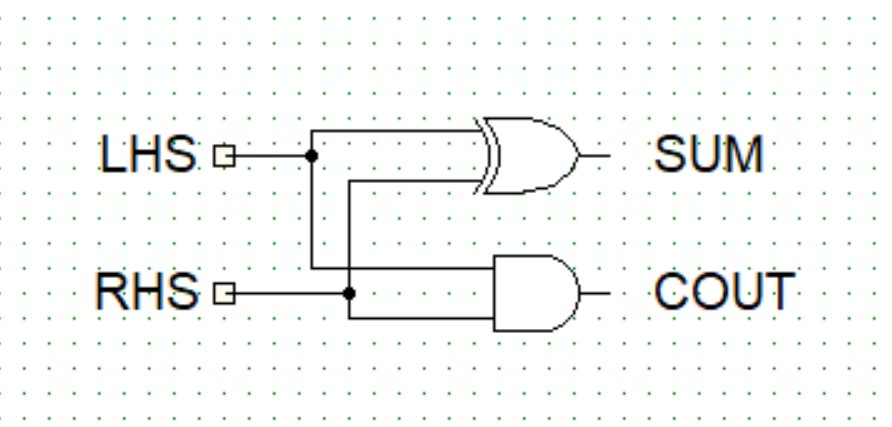
\includegraphics{images/one_bit_half_adder.jpg}
    \end{center}

    \begin{center}
      \begin{lstlisting}
        iverilog.exe src/one_bit_half_adder.v && vvp.exe a.out
        lhs = 0, rhs = 0, sum = 0, carry = 0
        lhs = 0, rhs = 1, sum = 1, carry = 0
        lhs = 1, rhs = 0, sum = 1, carry = 0
        lhs = 1, rhs = 1, sum = 0, carry = 1
      \end{lstlisting}
    \end{center}
  \end{problem}


  \begin{problem}{5}
    By cascading the sums of two half-adder modules and ORing the carries of
    both modules, a full adder can be constructed out of two simple half adders.

    \begin{center}
      \lstinputlisting{src/one_bit_full_adder.v}
    \end{center}

    \begin{center}
      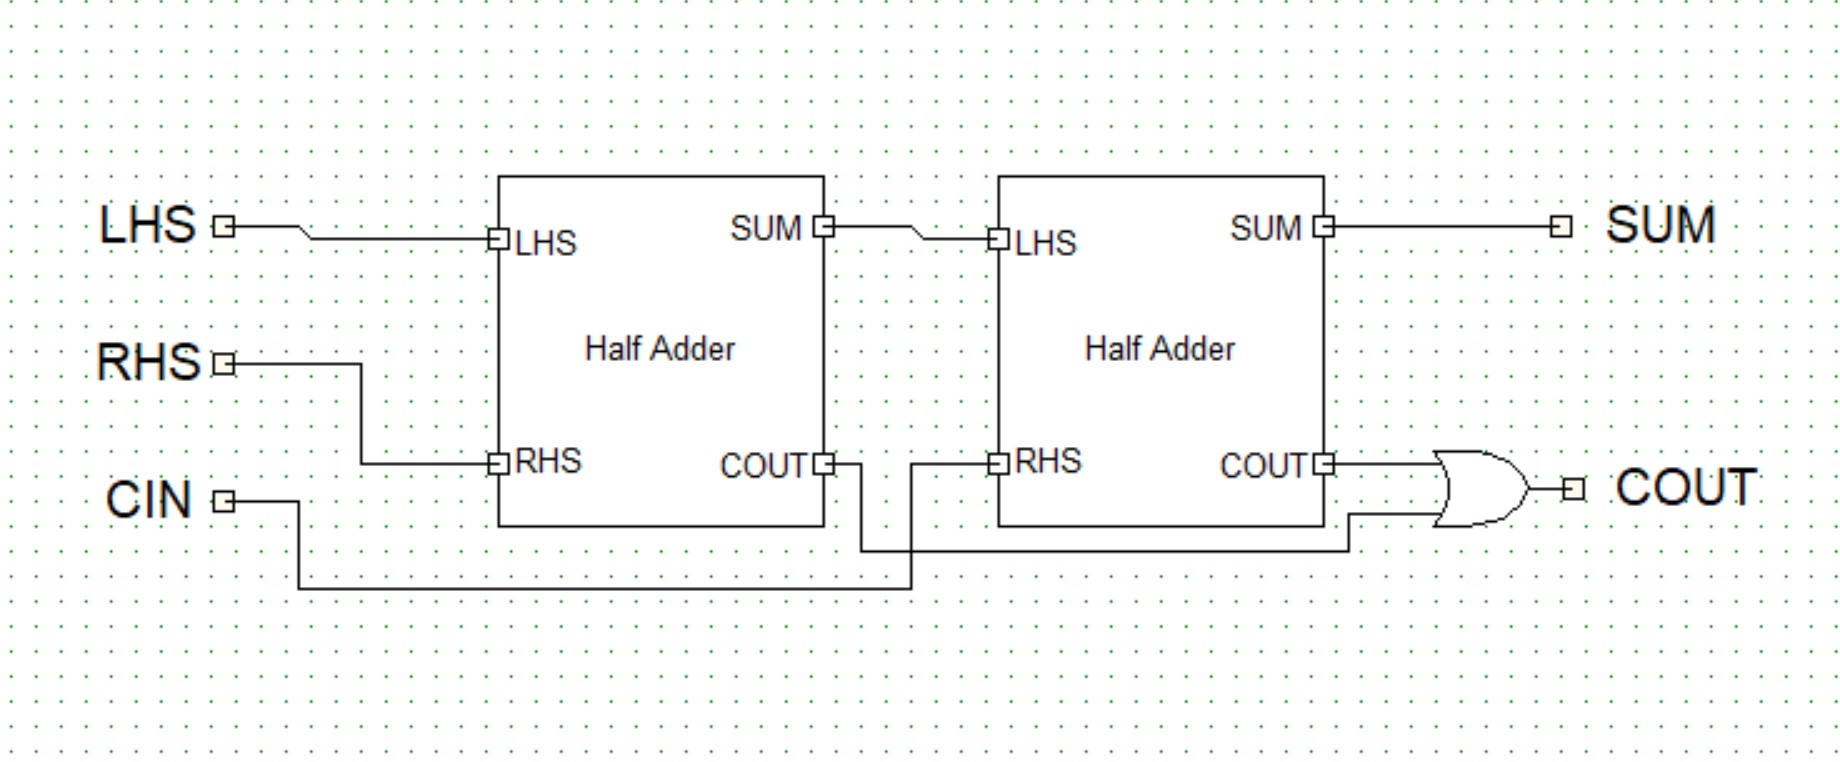
\includegraphics[scale=0.6]{images/one_bit_full_adder.jpg}
    \end{center}

    \begin{center}
      \begin{lstlisting}
        iverilog.exe src/one_bit_full_adder.v && vvp.exe a.out
        cin = 0, lhs = 0, rhs = 0, sum = 0, cout = 0
        cin = 0, lhs = 0, rhs = 1, sum = 1, cout = 0
        cin = 0, lhs = 1, rhs = 0, sum = 1, cout = 0
        cin = 0, lhs = 1, rhs = 1, sum = 0, cout = 1
        cin = 1, lhs = 0, rhs = 0, sum = 1, cout = 0
        cin = 1, lhs = 0, rhs = 1, sum = 0, cout = 1
        cin = 1, lhs = 1, rhs = 0, sum = 0, cout = 1
        cin = 1, lhs = 1, rhs = 1, sum = 1, cout = 1
      \end{lstlisting}
    \end{center}
  \end{problem}


  \begin{problem}{6}
    A full adder can be implemented directly (without chaining half-adders).
    The full adder takes three inputs (left-hand-side, right-hand-side, and
    carry-in). and produces sum and carry-out values.

    \begin{center}
      \begin{math}
        \begin{array}{ccc|cc}
          x&y&z&sum&cout\\\hline
          0&0&0&\mathbf{0}&\mathbf{0}\\
          0&0&1&\mathbf{1}&\mathbf{0}\\
          0&1&0&\mathbf{1}&\mathbf{0}\\
          0&1&1&\mathbf{0}&\mathbf{1}\\
          1&0&0&\mathbf{1}&\mathbf{0}\\
          1&0&1&\mathbf{0}&\mathbf{1}\\
          1&1&0&\mathbf{0}&\mathbf{1}\\
          1&1&1&\mathbf{1}&\mathbf{1}
        \end{array}
      \end{math}
    \end{center}

    \begin{center}
      \begin{karnaugh-map}[4][2][1][$yz$][$x$]
        \minterms{1, 2, 4, 7}
        \maxterms{0, 3, 5, 6}
        \implicant{1}{1}
        \implicant{2}{2}
        \implicant{4}{4}
        \implicant{7}{7}
      \end{karnaugh-map}
    \end{center}

    \begin{center}
      \begin{karnaugh-map}[4][2][1][$yz$][$x$]
        \minterms{3, 5, 6, 7}
        \maxterms{0, 1, 2, 4}
        \implicant{3}{7}
        \implicant{5}{7}
        \implicant{7}{6}
      \end{karnaugh-map}
    \end{center}

    \begin{center}
      \lstinputlisting{src/one_bit_full_adder_direct.v}
    \end{center}

    \begin{center}
      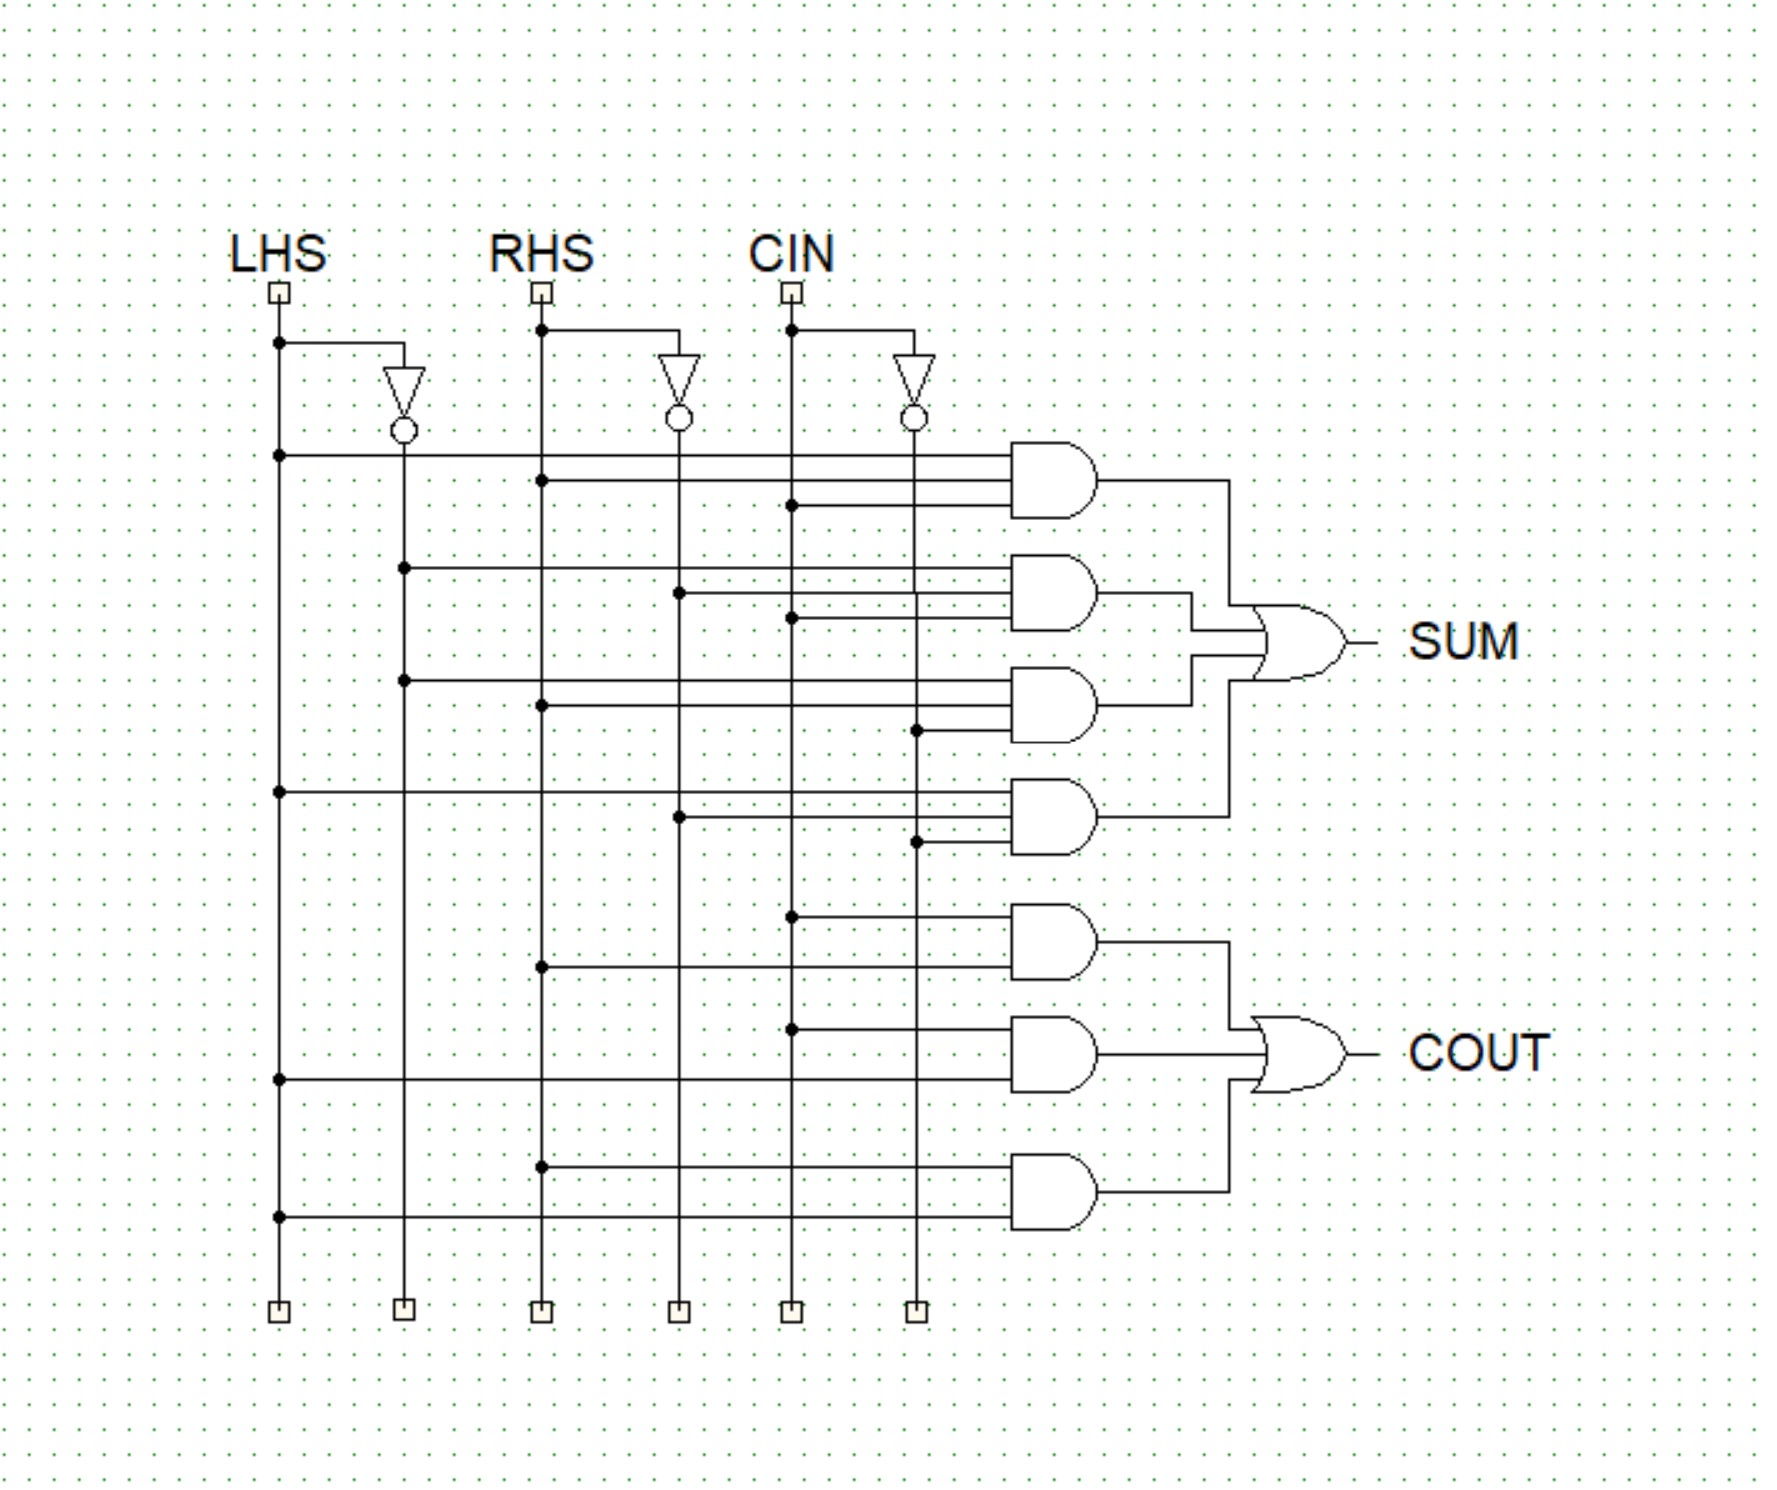
\includegraphics[scale=0.6]{images/one_bit_full_adder_direct.jpg}
    \end{center}

    \begin{center}
      \begin{lstlisting}
        iverilog.exe src/one_bit_full_adder_direct.v && vvp.exe a.out
        cin = 0, lhs = 0, rhs = 0, sum = 0, cout = 0
        cin = 0, lhs = 0, rhs = 1, sum = 1, cout = 0
        cin = 0, lhs = 1, rhs = 0, sum = 1, cout = 0
        cin = 0, lhs = 1, rhs = 1, sum = 0, cout = 1
        cin = 1, lhs = 0, rhs = 0, sum = 1, cout = 0
        cin = 1, lhs = 0, rhs = 1, sum = 0, cout = 1
        cin = 1, lhs = 1, rhs = 0, sum = 0, cout = 1
        cin = 1, lhs = 1, rhs = 1, sum = 1, cout = 1
      \end{lstlisting}
    \end{center}
  \end{problem}


  \begin{problem}{7}
    By using a control bit and XORing the right hand side, a cascaded adder can
    be used as a subtractor (by adding the 2's complement inverse).  By
    cascading four one-bit full adders, a four-bit adder/subtractor can be
    created.  If the c2 and cout lines have different values, then an overflow
    must have occured.

    \begin{center}
      \lstinputlisting{src/four_bit_adder.v}
    \end{center}

    \begin{center}
      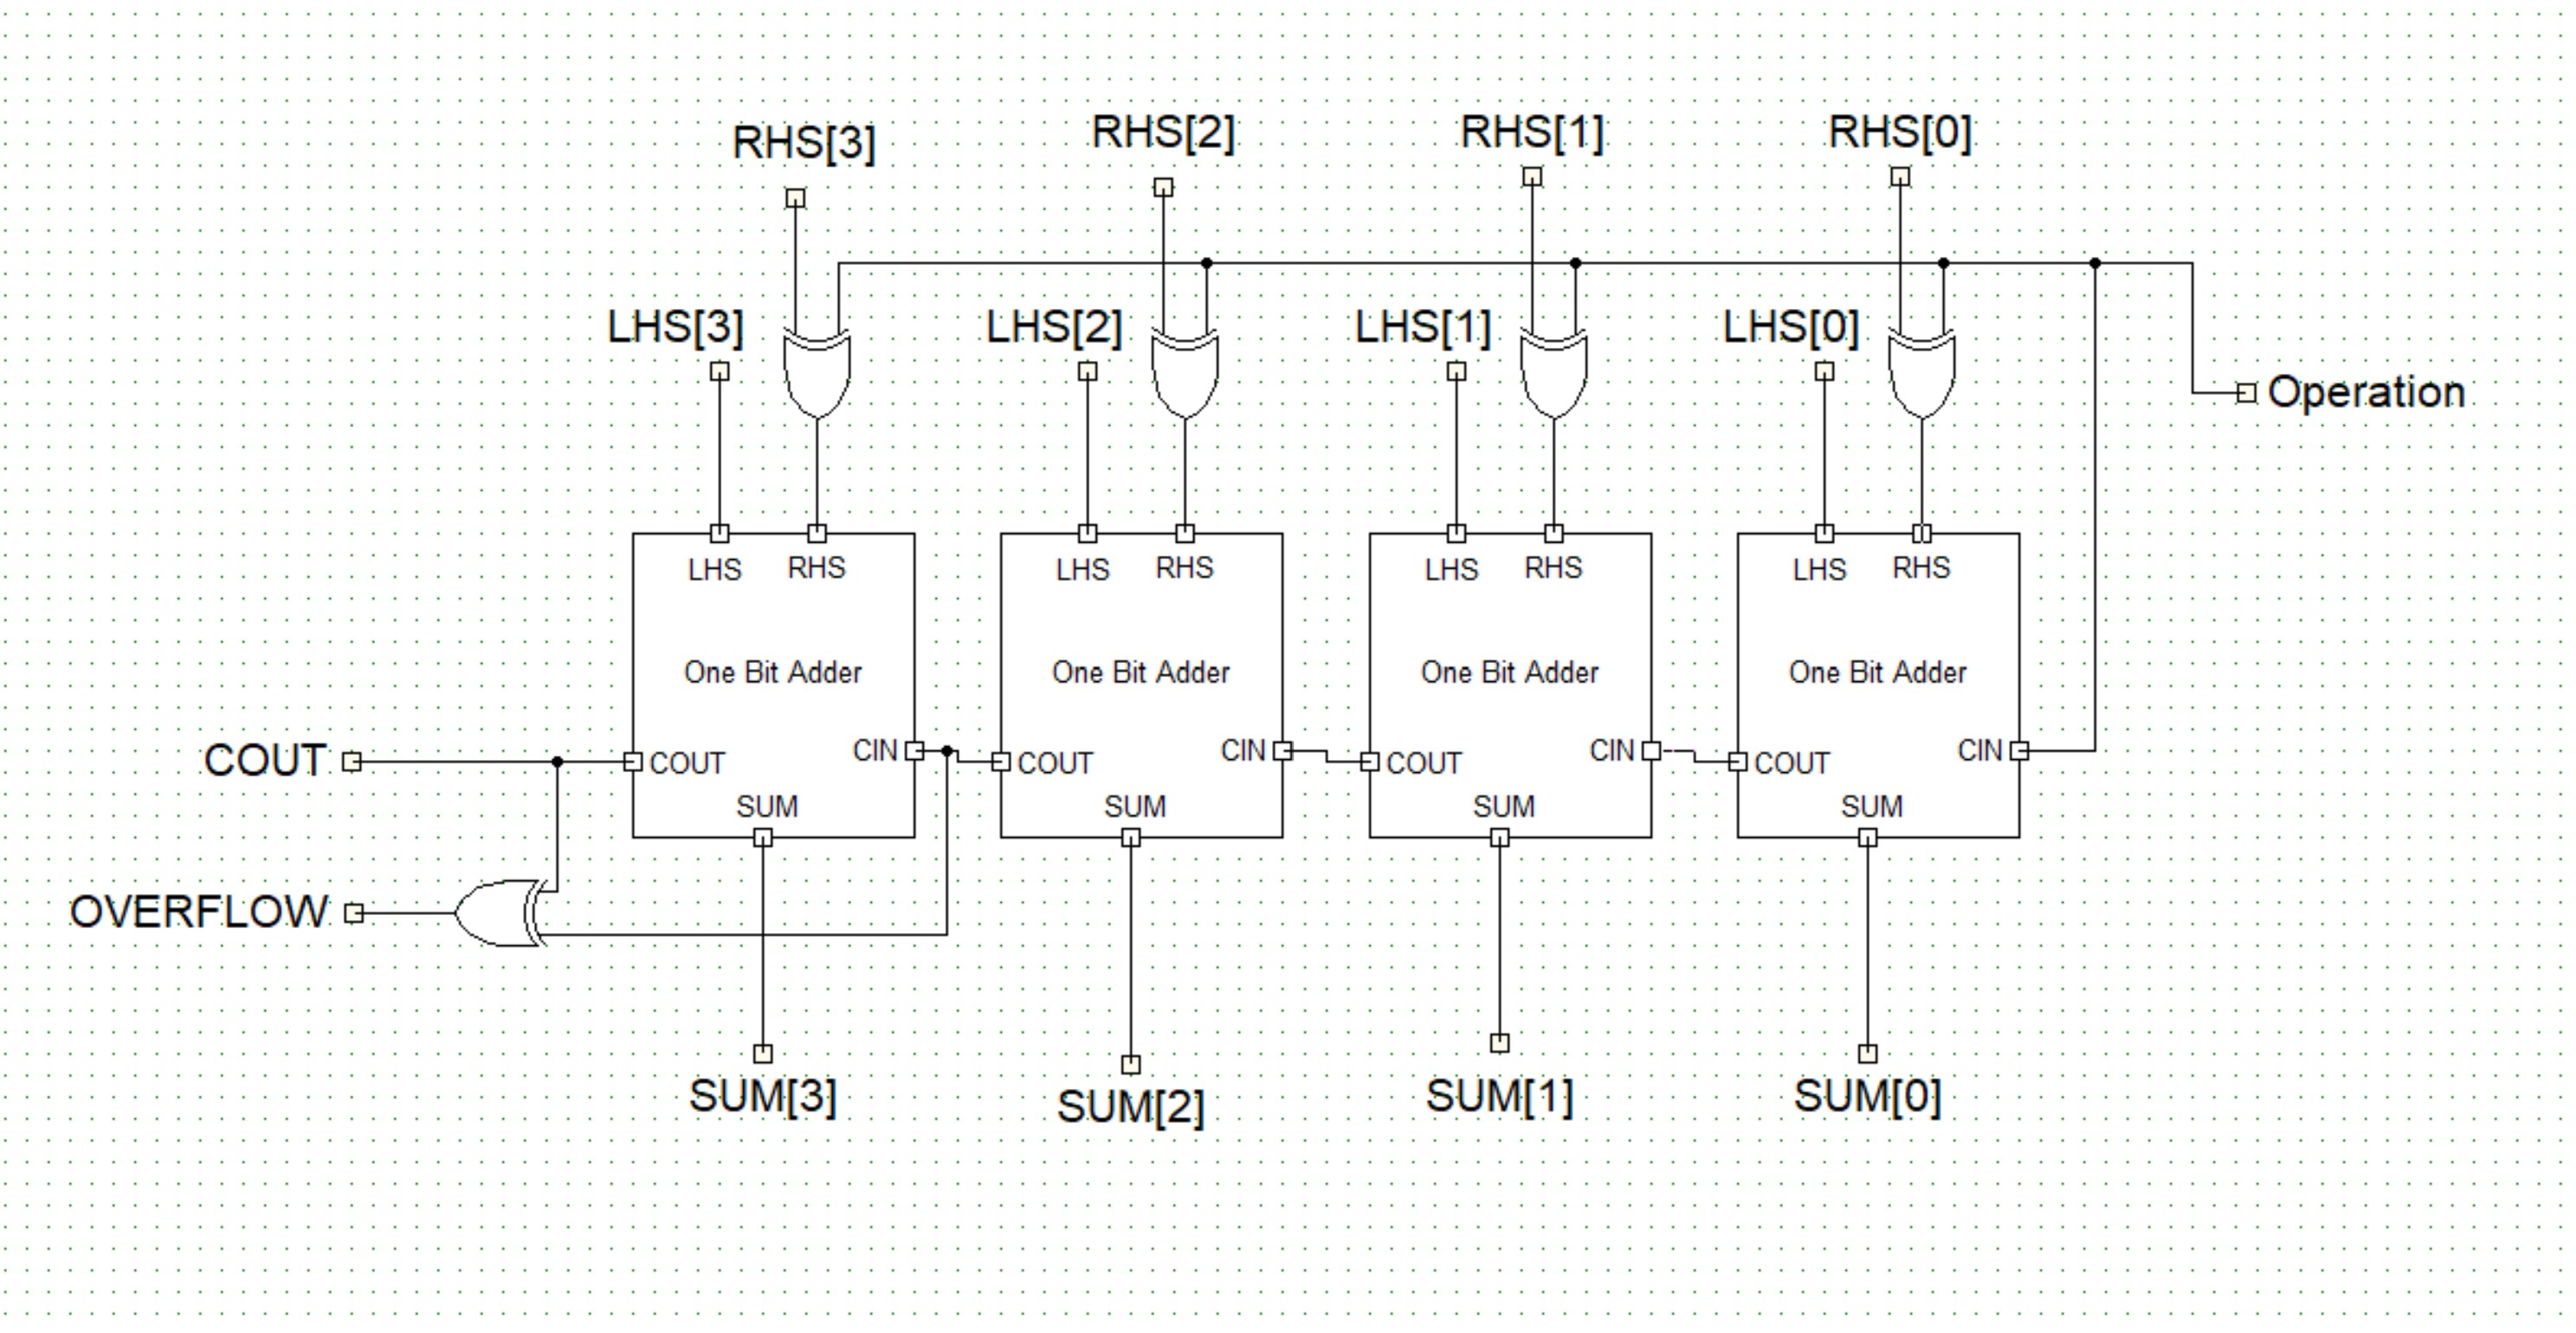
\includegraphics[scale=0.35]{images/four_bit_adder_subtractor.jpg}
    \end{center}

    \begin{center}
      \begin{lstlisting}
        iverilog.exe src/four_bit_adder.v && vvp.exe a.out
        op = 0, lhs =  5, rhs =  3, sum = -8, cout = 0, overflow = 1
        op = 0, lhs =  5, rhs =  0, sum =  5, cout = 0, overflow = 0
        op = 0, lhs =  5, rhs = -6, sum = -1, cout = 0, overflow = 0
        op = 1, lhs =  3, rhs = -3, sum =  6, cout = 0, overflow = 0
        op = 1, lhs =  4, rhs =  2, sum =  2, cout = 1, overflow = 0
        op = 0, lhs =  6, rhs =  7, sum = -3, cout = 0, overflow = 1
        op = 0, lhs =  0, rhs =  0, sum =  0, cout = 0, overflow = 0
        op = 1, lhs =  0, rhs =  0, sum =  0, cout = 1, overflow = 0
      \end{lstlisting}
    \end{center}
  \end{problem}


  \begin{problem}{Extra}
    The seven segment LED driver can be implemented as seven seperate functions,
    one for each segment of the LED display (a..g).
    
    \begin{center}
      \begin{math}
        \begin{array}{ccc|ccccccc}
          x&y&z&a&b&c&d&e&f&g\\\hline
          0&0&0&\mathbf{1}&\mathbf{1}&\mathbf{1}&\mathbf{1}&\mathbf{1}&\mathbf{1}&\mathbf{0}\\
          0&0&1&\mathbf{0}&\mathbf{1}&\mathbf{1}&\mathbf{0}&\mathbf{0}&\mathbf{0}&\mathbf{0}\\
          0&1&0&\mathbf{1}&\mathbf{0}&\mathbf{1}&\mathbf{1}&\mathbf{0}&\mathbf{1}&\mathbf{1}\\
          0&1&1&\mathbf{1}&\mathbf{0}&\mathbf{0}&\mathbf{1}&\mathbf{1}&\mathbf{1}&\mathbf{1}\\
          1&0&0&\mathbf{0}&\mathbf{1}&\mathbf{1}&\mathbf{0}&\mathbf{0}&\mathbf{1}&\mathbf{1}\\
          1&0&1&\mathbf{1}&\mathbf{1}&\mathbf{1}&\mathbf{1}&\mathbf{0}&\mathbf{1}&\mathbf{1}\\
          1&1&0&\mathbf{1}&\mathbf{0}&\mathbf{1}&\mathbf{1}&\mathbf{1}&\mathbf{1}&\mathbf{1}\\
          1&1&1&\mathbf{1}&\mathbf{1}&\mathbf{1}&\mathbf{0}&\mathbf{0}&\mathbf{0}&\mathbf{0}
        \end{array}
      \end{math}
    \end{center}

    \begin{center}
      \begin{karnaugh-map}[4][2][1][$yz$][$x$]
        \minterms{0, 2, 3, 5, 6, 7}
        \maxterms{1, 4}
        \implicant{3}{6}
        \implicant{5}{7}
        \implicantedge{0}{0}{2}{2}
      \end{karnaugh-map}
    \end{center}

    \begin{center}
      \begin{karnaugh-map}[4][2][1][$yz$][$x$]
        \minterms{0, 1, 4, 5, 7}
        \maxterms{2, 3, 6}
        \implicant{0}{5}
        \implicant{5}{7}
      \end{karnaugh-map}
    \end{center}

    \begin{center}
      \begin{karnaugh-map}[4][2][1][$yz$][$x$]
        \minterms{0, 1, 2, 4, 5, 6, 7}
        \maxterms{3}
        \implicant{0}{5}
        \implicant{4}{6}
        \implicantedge{0}{4}{2}{6}
      \end{karnaugh-map}
    \end{center}

    \begin{center}
      \begin{karnaugh-map}[4][2][1][$yz$][$x$]
        \minterms{0, 2, 3, 5, 6}
        \maxterms{1, 4, 7}
        \implicantedge{0}{0}{2}{2}
        \implicant{3}{2}
        \implicant{2}{6}
        \implicant{5}{5}
      \end{karnaugh-map}
    \end{center}

    \begin{center}
      \begin{karnaugh-map}[4][2][1][$yz$][$x$]
        \minterms{0, 3, 6}
        \maxterms{1, 2, 4, 5, 7}
        \implicant{0}{0}
        \implicant{3}{3}
        \implicant{6}{6}
      \end{karnaugh-map}
    \end{center}

    \begin{center}
      \begin{karnaugh-map}[4][2][1][$yz$][$x$]
        \minterms{0, 2, 3, 4, 5, 6}
        \maxterms{1, 7}
        \implicantedge{0}{4}{2}{6}
        \implicant{4}{5}
        \implicant{3}{2}
      \end{karnaugh-map}
    \end{center}

    \begin{center}
      \begin{karnaugh-map}[4][2][1][$yz$][$x$]
        \minterms{2, 3, 4, 5, 6}
        \maxterms{0, 1, 7}
        \implicant{4}{5}
        \implicant{3}{2}
        \implicant{2}{6}
      \end{karnaugh-map}
    \end{center}

    \begin{center}
      \lstinputlisting{src/seven_segment.v}
    \end{center}

    \begin{center}
      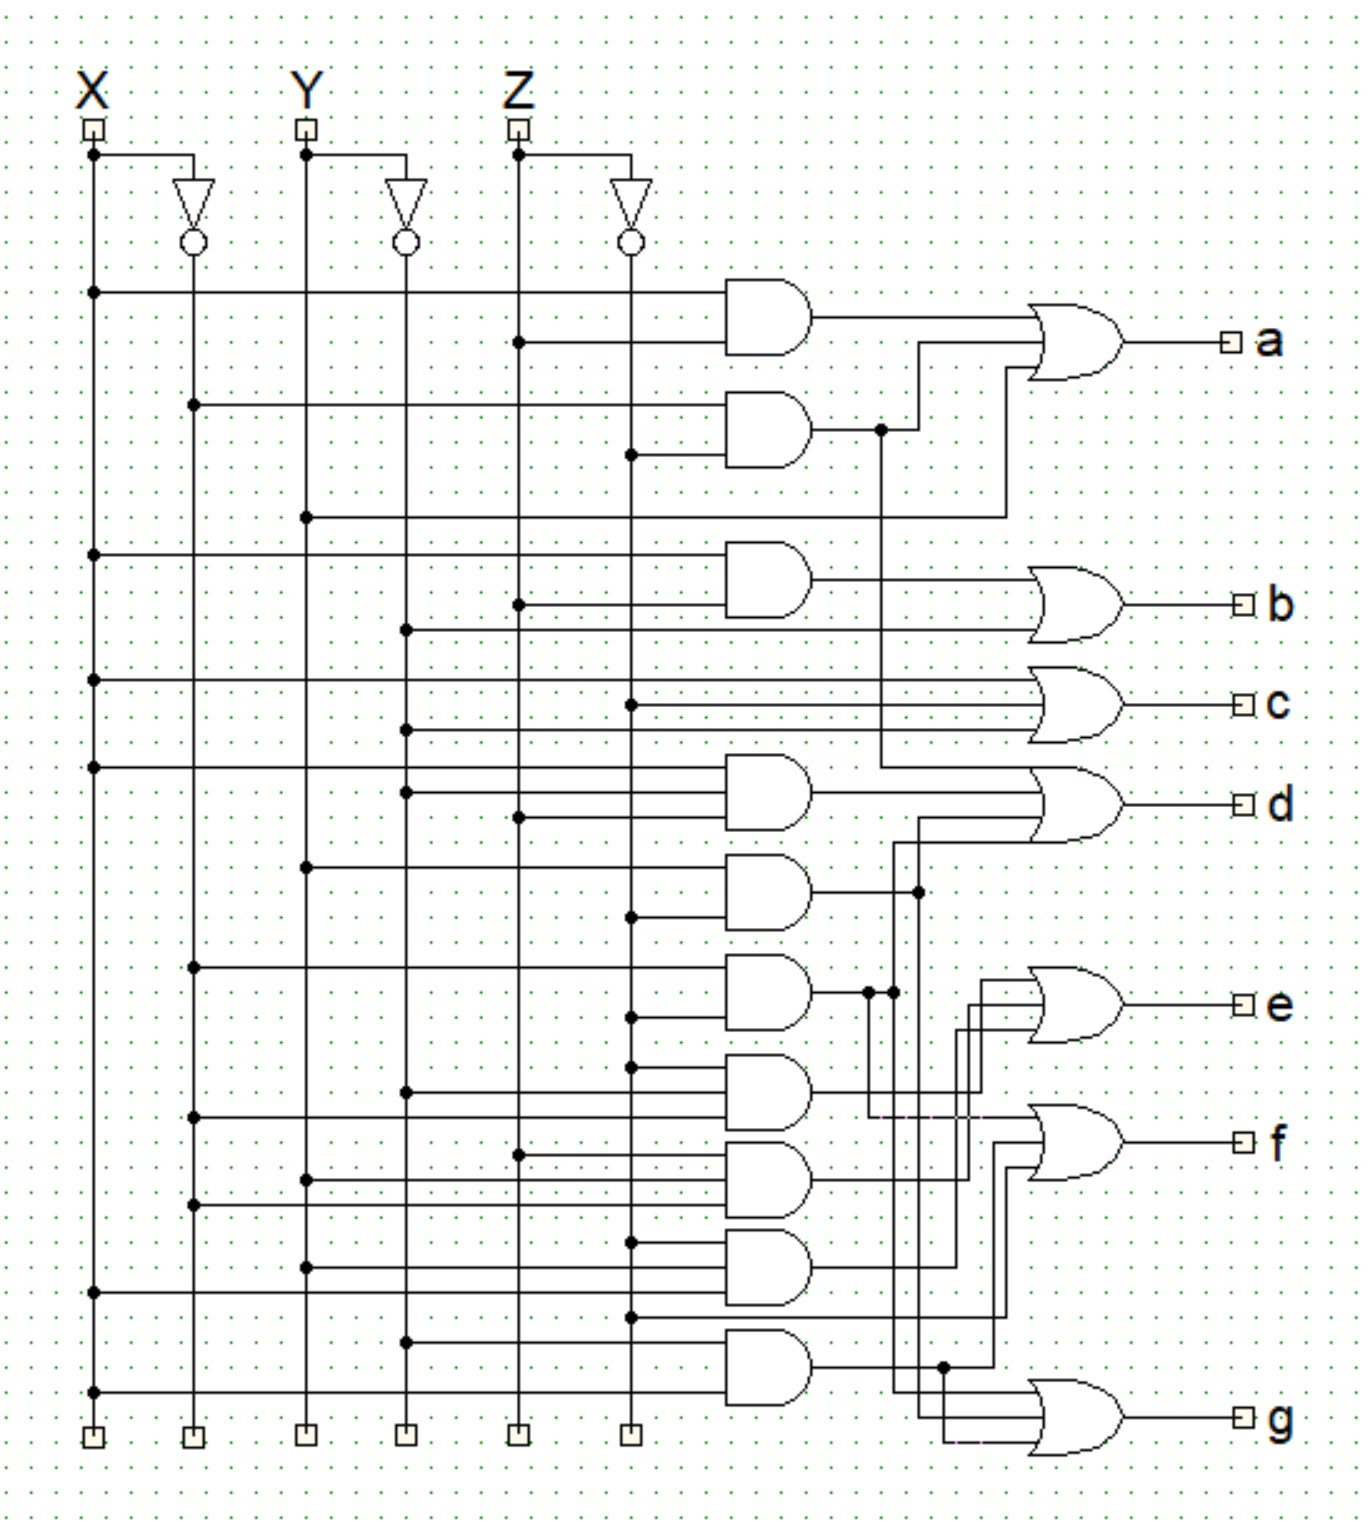
\includegraphics[scale=0.8]{images/seven_segment.jpg}
    \end{center}

    \begin{center}
      \begin{lstlisting}
        iverilog.exe src/seven_segment.v && vvp.exe a.out
        x = 0, y = 0, z = 0, a = 1, b = 1, c = 1, d = 1, e = 1, f = 1, g = 0
        x = 0, y = 0, z = 1, a = 0, b = 1, c = 1, d = 0, e = 0, f = 0, g = 0
        x = 0, y = 1, z = 0, a = 1, b = 0, c = 1, d = 1, e = 0, f = 1, g = 1
        x = 0, y = 1, z = 1, a = 1, b = 0, c = 0, d = 1, e = 1, f = 1, g = 1
        x = 1, y = 0, z = 0, a = 0, b = 1, c = 1, d = 0, e = 0, f = 1, g = 1
        x = 1, y = 0, z = 1, a = 1, b = 1, c = 1, d = 1, e = 0, f = 1, g = 1
        x = 1, y = 1, z = 0, a = 1, b = 0, c = 1, d = 1, e = 1, f = 1, g = 1
        x = 1, y = 1, z = 1, a = 1, b = 1, c = 1, d = 0, e = 0, f = 0, g = 0
      \end{lstlisting}
    \end{center}
  \end{problem}
\end{document}